
\documentclass{beamer}

\usetheme{focus} % see https://github.com/elauksap/focus-beamertheme
% Add option [numbering=none] to disable the footer progress bar
% Add option [numbering=fullbar] to show the footer progress bar as always full with a slide count

\usepackage{booktabs} % Required for better table rules
\usepackage{bm,times}

\newcommand{\eps}{\epsilon}
\newcommand{\RR}{\mathbb{R}}

\newcommand{\grad}{\nabla}
\newcommand{\Div}{\nabla\cdot}
\newcommand{\trace}{\operatorname{tr}}

\newcommand{\hbn}{\hat{\mathbf{n}}}

\newcommand{\bb}{\mathbf{b}}
\newcommand{\be}{\mathbf{e}}
\newcommand{\bbf}{\mathbf{f}}
\newcommand{\bg}{\mathbf{g}}
\newcommand{\bn}{\mathbf{n}}
\newcommand{\br}{\mathbf{r}}
\newcommand{\bu}{\mathbf{u}}
\newcommand{\bv}{\mathbf{v}}
\newcommand{\bw}{\mathbf{w}}
\newcommand{\bx}{\mathbf{x}}

\newcommand{\bF}{\mathbf{F}}
\newcommand{\bV}{\mathbf{V}}
\newcommand{\bX}{\mathbf{X}}

\newcommand{\bxi}{\bm{\xi}}

\newcommand{\bzero}{\bm{0}}

\newcommand{\rhoi}{\rho_{\text{i}}}

\newcommand{\ip}[2]{\left(#1,#2\right)}

\newcommand{\mR}{R^{\bm{\oplus}}}
\newcommand{\iR}{R^{\bullet}}

\newcommand{\pp}{{\text{p}}}
\newcommand{\qq}{{\text{q}}}
\newcommand{\rr}{{\text{r}}}

\newcommand{\bus}{\bu|_s}


\title{Evolution of Ice Sheet Geometry using Stokes Dynamics}

%\subtitle{Subtitle}

\author{Ed Bueler}

\titlegraphic{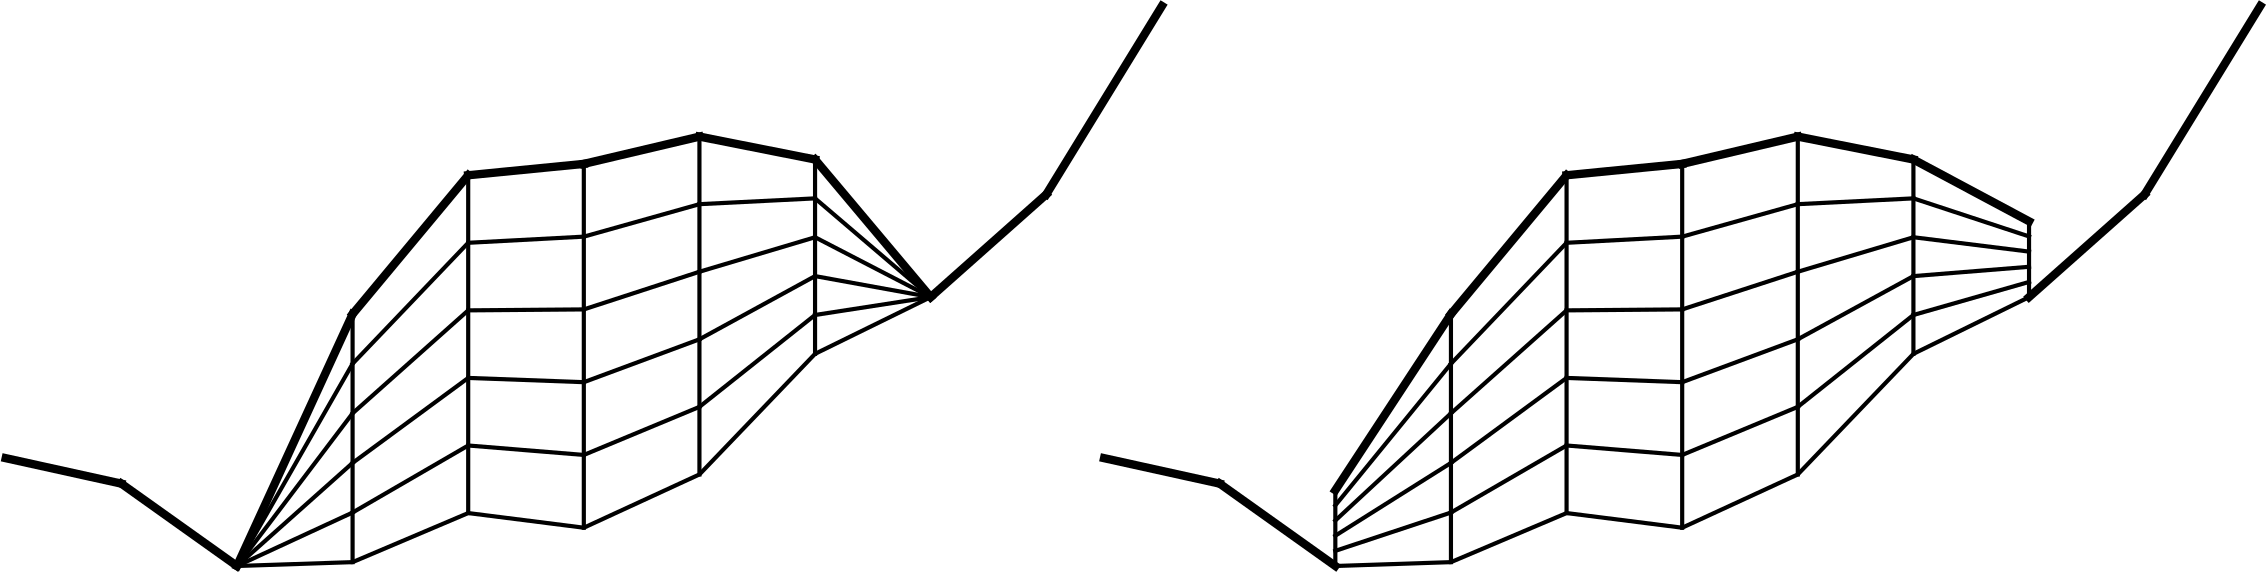
\includegraphics[width=0.55\textwidth]{figs/extruded.png} \\ 
\includegraphics[width=0.18\textwidth]{figs/uafbw.png}}

\institute{University of Alaska Fairbanks}

\date{\phantom{foo} \bigskip \bigskip \\ SIAM GS21 \\ with assistance from Lawrence Mitchell}


\begin{document}

\begin{frame}
	\maketitle
\end{frame}


\begin{frame}{the steady ice geometry problem (SIGP)}

\vspace{-2mm}
\begin{center}
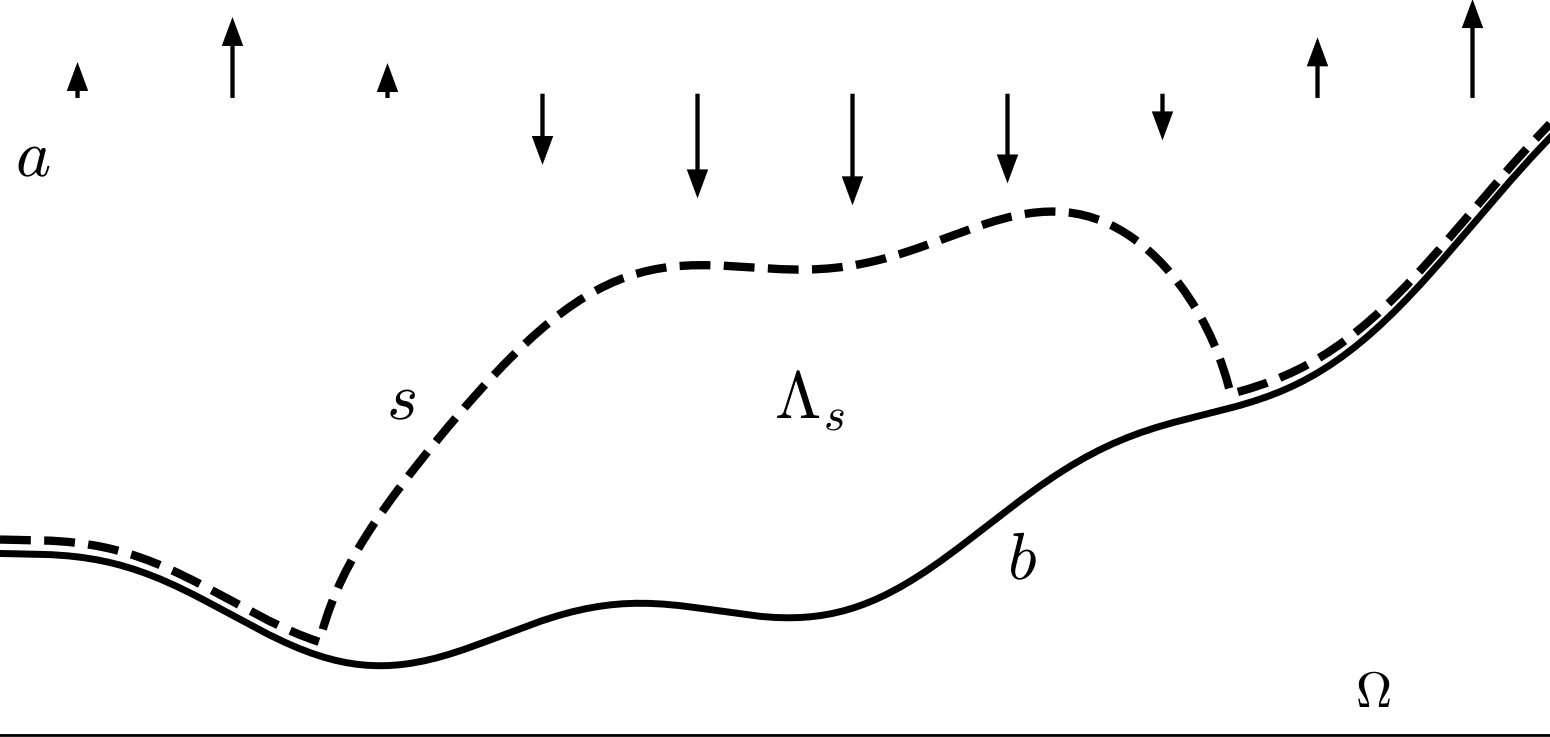
\includegraphics[width=0.7\textwidth]{figs/stokesdomain.png}
\end{center}

\vspace{-1mm}
\begin{itemize}
\item a non-shallow glacier interacting with the climate
    \begin{itemize}
    \item the simplest such problem (nonsliding, isothermal)
    \item re~\emph{steady}: solve it and you can handle implicit steps too
    \end{itemize}
\item data given on fixed $\Omega \subset \RR^2$:
    \begin{itemize}
    \item climatic mass balance $a(x,y)$ \hfill $\gets$ \emph{steady climate}
    \item bed elevation $b(x,y)$
    \end{itemize}
\item \emph{determine surface elevation $s(x,y)$ on $\Omega$ and domain $\Lambda_s \subset \RR^3$}
\end{itemize}
\end{frame}


\begin{frame}{SIGP strong form}

\begin{itemize}
\item \alert{a nonlinear complementarity problem (NCP) coupled to the Glen-Stokes model for ice velocity $\bu$:}

\vspace{-2mm}
\begin{align*}
s - b &\ge 0 && \text{on $\Omega$} \\
- \bu|_s \cdot \bn_s - a &\ge 0 && \text{''} \\
(s - b) (- \bu|_s \cdot \bn_s - a) &= 0 && \text{''} \\
- \nabla \cdot \left(2 \nu_\eps\, D\bu\right) + \nabla p - \rhoi \mathbf{g} &= \bzero && \text{on $\Lambda_s$} \\
\nabla \cdot \bu &= 0 && \text{''} \\
\left(2 \nu_\eps D\bu - pI\right) \bn &= \bzero && \text{on $\partial \Lambda_s \setminus \Gamma_0$} \\
\bu &= \bzero && \text{on $\Gamma_0$ (ice base)}
\end{align*}

    \begin{itemize}
    \item Glen-law effective viscosity with $\text{p}=(1/\text{n})+1=4/3$:
      $$\nu_\eps = \frac{1}{2} B_n \left(|D\bu|^2 + \eps\, D_0^2\right)^{(\pp-2)/2}$$
    \item surface kinematical equation holds \emph{on the ice}: \quad $\bu|_s \cdot \bn_s + a=0$
    \end{itemize}
\end{itemize}
\end{frame}


\begin{frame}{what do existing ice sheet models do?}

FIXME screenshot from Seguinot

\begin{itemize}
\item almost no one is addressing the SIGP directly
    \begin{itemize}
    \item except \cite{WirbelJarosch2020}, but nonscalably and with ``fake ice'' extension
    \item note scalable solution of fixed-geometry Glen-Stokes by Isaac and others \cite{IsaacStadlerGhattas2015}
    \end{itemize}
\item \emph{warning}: this free boundary problem is a barrier to exact numerical mass conservation, regardless of dynamical and/or numerical choices \cite{Bueler2021conservation}
\item what are people doing?  \emph{explicit time-stepping with $s \ge b$ enforced by truncation}
\item \alert{show movie clip}
\end{itemize}
\end{frame}


\begin{frame}{new method}

\begin{itemize}
\item FIXME \cite{BuelerMitchell2022}
\end{itemize}
\end{frame}



%\begin{block}{Block}
%\begin{alertblock}{Alert block}
%	\pause % Automatically creates a new "page" split between the above and above + below
%	\begin{exampleblock}{Example block}


%\begin{frame}{Columns}
%	\begin{columns}
%		\column{0.5\textwidth}
%			This text
%		\column{0.5\textwidth}
%			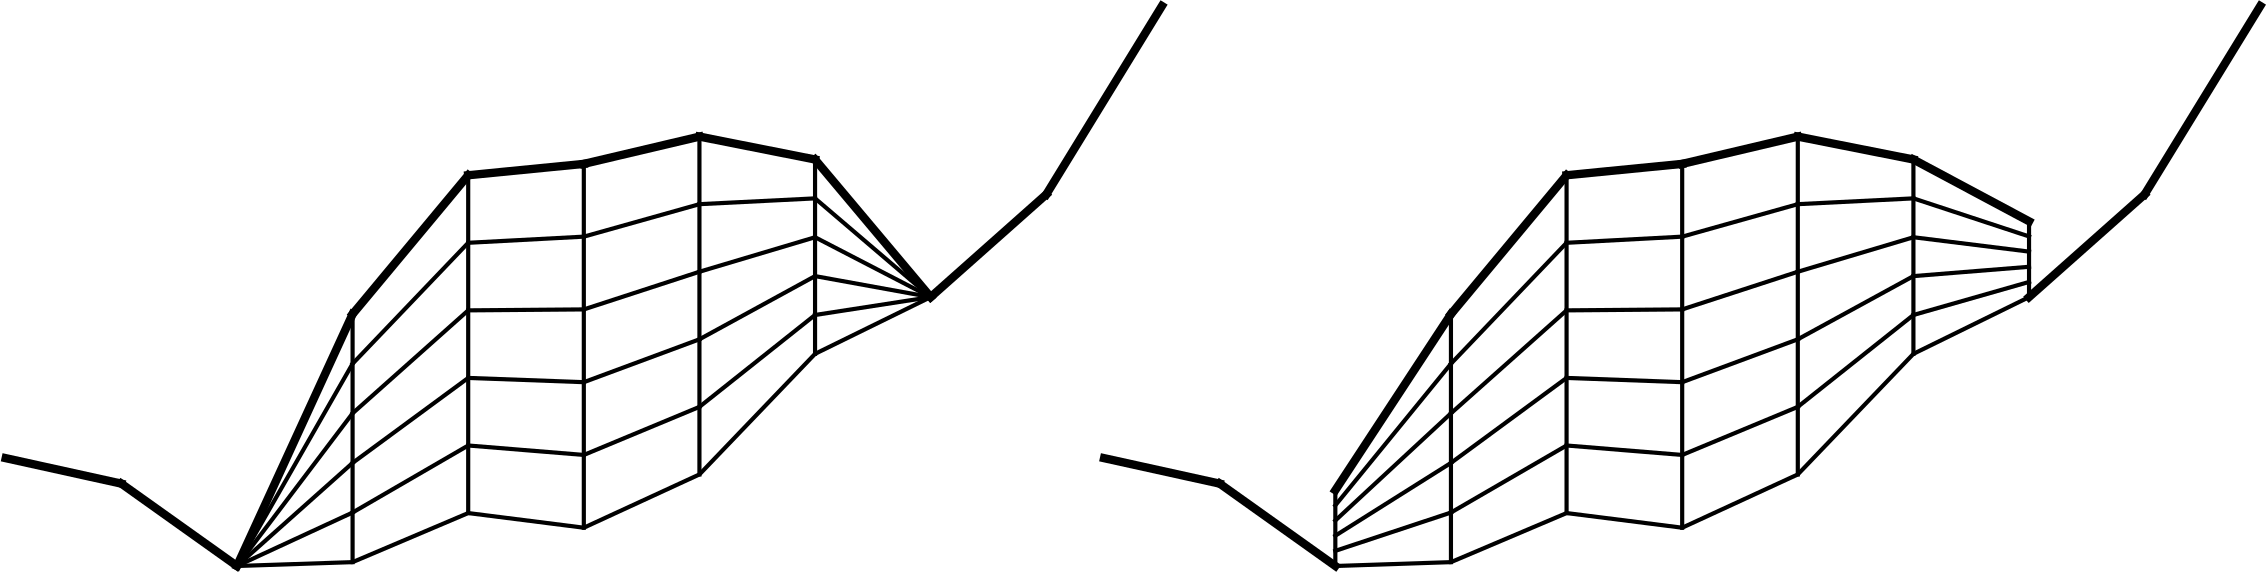
\includegraphics[width=\linewidth]{figs/extruded.png}
%	\end{columns}
%\end{frame}


\appendix

\begin{frame}{References}
	\bibliography{../paper/msg.bib}
	\bibliographystyle{plain}
\end{frame}


\end{document}
